%%%%%%%%%%%%%%%%%%%%%%%%%%%%%%%%%%%%%%%%%%%%%%%%%%%%%%%%%%%%%%%%%%%%%%%%%
%                                                                       %
% ustthesis_test.tex: A template file for usage with ustthesis.cls      %
%                                                                       %
%%%%%%%%%%%%%%%%%%%%%%%%%%%%%%%%%%%%%%%%%%%%%%%%%%%%%%%%%%%%%%%%%%%%%%%%%

\documentclass{ustthesis}

\usepackage{times,amsmath,epsfig}
\usepackage{graphicx,algorithm}
\usepackage[noend]{algorithmic}
\usepackage[center]{subfigure}
\usepackage{color,graphicx}
\usepackage{amsmath}
\newtheorem{proof}{Proof}
\usepackage[left=2.5cm,top=0.21cm,bottom=0.21cm,right=2.5cm]{geometry}
 
\newcommand{\red}[1]{#1}
\newcommand{\tab}[1]{\hspace{3mm}}

% \usepackage{latexsym}
    % Use the "latexsym" package when encountering the following error:
    %   ! LaTeX Error: Command \??? not provided in base LaTeX2e.
% \usepackage{epsf}
    % Use the "epsf" package for including EPS files.

%%%%%%%%%%%%%%%%%%%%%%%%%%%%%%%%%%%%%%%%%%%%%%%%%%%%%%%%%%%%%%%%%%%%%%%%%
%                                                                       %
% Preambles. DO NOT ERASE THEM. Change to suite your particular purpose.%
%                                                                       %
%%%%%%%%%%%%%%%%%%%%%%%%%%%%%%%%%%%%%%%%%%%%%%%%%%%%%%%%%%%%%%%%%%%%%%%%%

\title{Master Thesis Proposal}  % Title of the thesis.
\author{San~Zhang}     % Author of the thesis.
\degree{\MPhil}             % Degree for which the thesis is.
%% or
%\degree{\PhD}              % Degree for which the thesis is.
\subject{Division of the RBM}      % Subject of the Degree.
\department{Information Hub}       % Department to which the thesis
                    % is submitted.
\advisor{Associate Prof. x }     % Supervisor.
\depthead{Prof.~xx}    % department head.
\defencedate{2023}{02}{04}      % \defencedate{year}{month}{day}.

% NOTE:
%   According to the sample shown in the guidelines, page number is
%   placed below the bottom margin.  However, if the author prefers
%   the page number to be printed above the bottom margin, please
%   activate the following command.

% \PNumberAboveBottomMargin

\begin{document}

%%%%%%%%%%%%%%%%%%%%%%%%%%%%%%%%%%%%%%%%%%%%%%%%%%%%%%%%%%%%%%%%%%%%%%%%%
%                                                                       %
% Now the actual Thesis. The order of output MUST be followed:          %
%                                                                       %
%    1) TITLEPAGE                                                       %
%                                                                       %
% The \maketitle command generates the Title page as well as the        %
% Signature page.                                                       %
%                                                                       %
%%%%%%%%%%%%%%%%%%%%%%%%%%%%%%%%%%%%%%%%%%%%%%%%%%%%%%%%%%%%%%%%%%%%%%%%%

\maketitle

%%%%%%%%%%%%%%%%%%%%%%%%%%%%%%%%%%%%%%%%%%%%%%%%%%%%%%%%%%%%%%%%%%%%%%%%%
%                                                                       %
%     2) DEDICATION (Optional)                                          %
%                                                                       %
% The \dedication and \enddedication commands are optional. If          %
% specified it generates a page for dedication.                         %
%
%%%%%%%%%%%%%%%%%%%%%%%%%%%%%%%%%%%%%%%%%%%%%%%%%%%%%%%%%%%%%%%%%%%%%%%%%

% \dedication
% This is an optional section.
% \enddedication

%%%%%%%%%%%%%%%%%%%%%%%%%%%%%%%%%%%%%%%%%%%%%%%%%%%%%%%%%%%%%%%%%%%%%%%%%
%                                                                       %
%     3) ACKNOWLEDGMENTS                                                %
%                                                                       %
% \acknowledgments and \endacknowledgments defines the                  %
% Acknowledgments of the author of the Thesis.                          %
%                                                                       %
%%%%%%%%%%%%%%%%%%%%%%%%%%%%%%%%%%%%%%%%%%%%%%%%%%%%%%%%%%%%%%%%%%%%%%%%%


%%%%%%%%%%%%%%%%%%%%%%%%%%%%%%%%%%%%%%%%%%%%%%%%%%%%%%%%%%%%%%%%%%%%%%%%%
%                                                                       %
%     4) TABLE OF CONTENTS                                              %
%                                                                       %
%%%%%%%%%%%%%%%%%%%%%%%%%%%%%%%%%%%%%%%%%%%%%%%%%%%%%%%%%%%%%%%%%%%%%%%%%

\tableofcontents

%%%%%%%%%%%%%%%%%%%%%%%%%%%%%%%%%%%%%%%%%%%%%%%%%%%%%%%%%%%%%%%%%%%%%%%%%
%                                                                       %
%     5) LIST OF FIGURES (If Any)                                       %
%                                                                       %
%%%%%%%%%%%%%%%%%%%%%%%%%%%%%%%%%%%%%%%%%%%%%%%%%%%%%%%%%%%%%%%%%%%%%%%%%

\listoffigures

%%%%%%%%%%%%%%%%%%%%%%%%%%%%%%%%%%%%%%%%%%%%%%%%%%%%%%%%%%%%%%%%%%%%%%%%%
%                                                                       %
%     6) LIST OF TABLES (If Any)
%                                                                       %
%%%%%%%%%%%%%%%%%%%%%%%%%%%%%%%%%%%%%%%%%%%%%%%%%%%%%%%%%%%%%%%%%%%%%%%%%

\listoftables

%%%%%%%%%%%%%%%%%%%%%%%%%%%%%%%%%%%%%%%%%%%%%%%%%%%%%%%%%%%%%%%%%%%%%%%%%
%                                                                       %
%     7) ABSTRACT                                                       %
%                                                                       %
% \abstract and \endabstract are used to define a short Abstract for    %
% the Thesis.                                                           %
%                                                                       %
%%%%%%%%%%%%%%%%%%%%%%%%%%%%%%%%%%%%%%%%%%%%%%%%%%%%%%%%%%%%%%%%%%%%%%%%%

\begin{abstract}
This is abstract
\end{abstract}


%%%%%%%%%%%%%%%%%%%%%%%%%%%%%%%%%%%%%%%%%%%%%%%%%%%%%%%%%%%%%%%%%%%%%%%%%
%                                                                       %
%     8) The Actual Contents                                            %
%                                                                       %
% The command \chapters MUST BE USED to ensure that the entire content  %
% of the Thesis is double-spaced (in version 1.0).                      %
%                                                                       %
% However, in version 2.0, \chapters will be automatically added in     %
% the beginning of the first chapter.                                   %
%                                                                       %
%%%%%%%%%%%%%%%%%%%%%%%%%%%%%%%%%%%%%%%%%%%%%%%%%%%%%%%%%%%%%%%%%%%%%%%%%

%%\chapters         % Not necessary with ustthesis.cls (v2.0).

%%%%%%%%%%%%%%%%%%%%%%%%%%%%%%%%%%%%%%%%%%%%%%%%%%%%%%%%%%%%%%%%%%%%%%%%%
%                                                                       %
% Each chapter is defined via the \chapter command. The usual sectional %
% commands of LaTeX are also available.                                 %
%                                                                       %
%%%%%%%%%%%%%%%%%%%%%%%%%%%%%%%%%%%%%%%%%%%%%%%%%%%%%%%%%%%%%%%%%%%%%%%%%

\chapter{Source of research topic, research purpose and significance}\label{sec-source}

\section{The source of the topic}

An example of figure

\begin{figure}[ht]
  \centering
  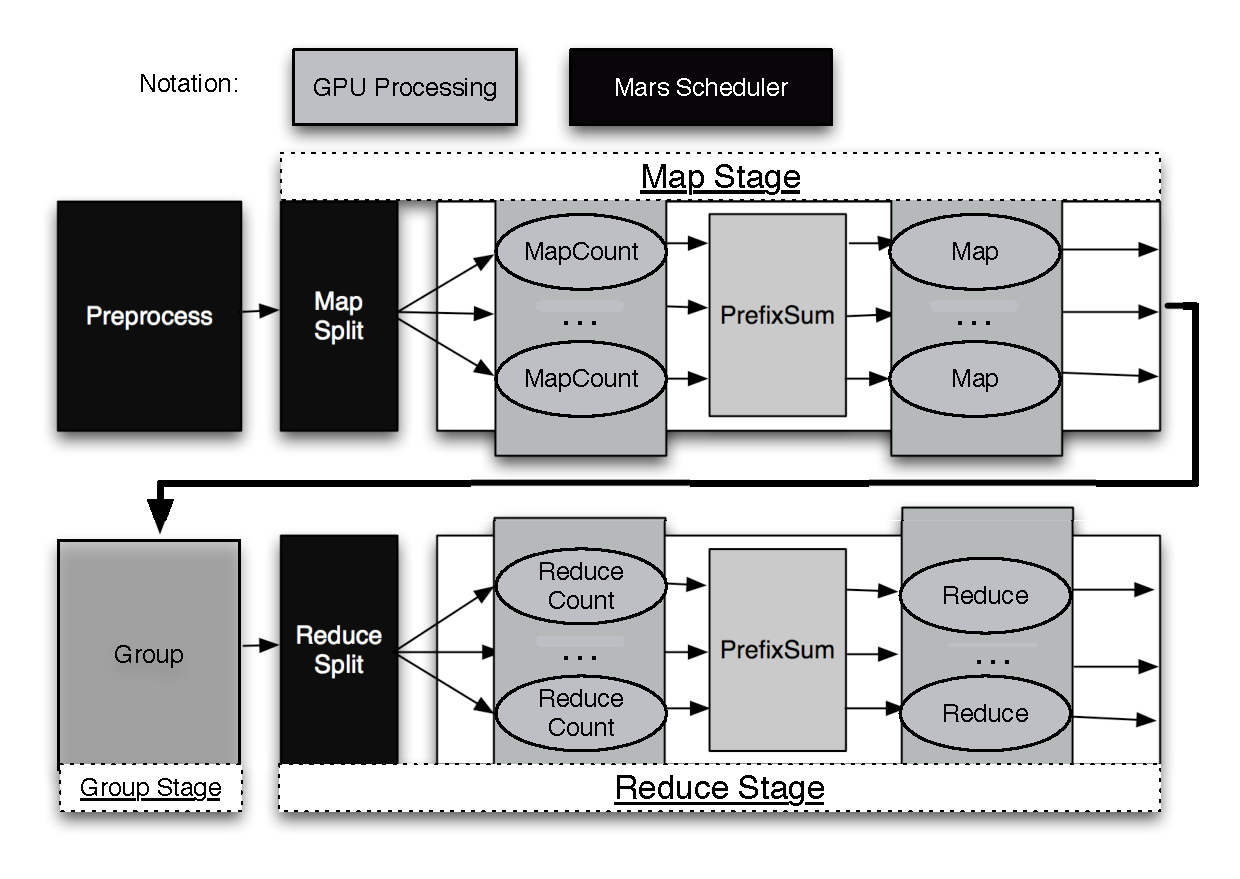
\includegraphics[width=0.60\textwidth]{figure/Mars_workflow.eps}
  \caption{The workflow of Mars on the GPU. }\label{fig:MarsWorkflow}
\end{figure}

{\em 1. Results on MarsBrook}



\doublerulesep 0.1pt
\begin{table}[htb]
  \centering
 \linespread{1.7}{ {\footnotesize
  \caption{Comparison on code sizes of MM and SS using MarsBrook and Brook+.}\label{tab:brookcodesize}
\vspace{2em}
  \begin{tabular}{ccc}
  \hline
\noalign{\smallskip}
  \textbf{Applications} & \textbf{MarsBrook} & \textbf{Brook+} \\
\noalign{\smallskip}
  \hline
  MM & 66 & 93 \\
  SS & 66 & 611  \\
  \hline
\noalign{\smallskip}
  \end{tabular}
  }}
\end{table}


\section{Research background and significance}

\textbf{Organization:} The remainder of the thesis is organized as
follows. We give a brief overview of GPUs, and review prior work on GPGPU and
MapReduce in Chapter~\ref{sec-preliminaries}. We present the design
and implementation details of Mars in Chapter~\ref{sec-design} and
Chapter~\ref{sec-implement} respectively. We present the extension
to multiple machines in
Chapter~\ref{sec-beyond}. In Chapter~\ref{sec-eval}, we present our
experimental results. Finally, we conclude in Chapter~\ref{sec-conclusion}.

\newpage

\chapter{Literature review and analysis}\label{sec-literature}

\section{Research review}
An examples


MapReduce is a successful paradigm~\cite{Dean2008}, originally proposed by Google,
for the ease of distributed data processing on a large number of machines.
In such a system, users specify two functions:
(1) a {\em map} function to process an input key/value pair,
and to generate a set of intermediate key/value pairs;
\section{Analysis of the literature review}
\newpage

\chapter{Main content of research}\label{sec-main-content}

xxx

\newpage

\chapter{Accomplished work}\label{sec-accomplished}


\newpage

\chapter{Research plan, expected objectives and results}\label{sec-RP}

\section{Research Plan} 
\section{Expected objectives and research achievements}
\section{ Time scheme}

\newpage

\chapter{Required conditions and resources}\label{sec-req-resources}

x

\newpage

\chapter{Anticipated problems and solutions}\label{sec-anticipated}


\newpage

\chapter{Conclusion}\label{sec-conclusion}

This is conclusion if need

%%%%%%%%%%%%%%%%%%%%%%%%%%%%%%%%%%%%%%%%%%%%%%%%%%%%%%%%%%%%%%%%%%%%%%%%%
%                                                                       %
%      9) BIBLIOGRAPHY                                                  %
%                                                                       %
% This example uses bibtex to generate the required Bibliography. Refer %
% to the % the file ustthesis_test.bib for the entries of the           %
% Bibliography. Note that only the cited entries are printed.           %
%                                                                       %
% If BibTeX is not used to typeset the bibliography, replace the        %
% following line with the \begin{thebibliography} and \end{bibliography}%
% commands (the "thebibliography" environment) to process the           %
% Bibliography.                                                         %
%                                                                       %
%%%%%%%%%%%%%%%%%%%%%%%%%%%%%%%%%%%%%%%%%%%%%%%%%%%%%%%%%%%%%%%%%%%%%%%%%

%%%%%%%%%%%%%%%%%%%%%%%%%%%%%%%%%%%%%%%%%%%%%%%%%%%%%%%%%%%%%%%%%%%%%%%%%
%                                                                       %
% The recommended bibliography style is the IEEE bibliography style.    %
% "ustbib" defines the IEEE bibliography standard with the added        %
% ability of sorting the items by name of author.                       %
%                                                                       %
% If you are not using BibTeX to process your Bibliography, comment out %
% the following line.                                                   %
%                                                                       %
%%%%%%%%%%%%%%%%%%%%%%%%%%%%%%%%%%%%%%%%%%%%%%%%%%%%%%%%%%%%%%%%%%%%%%%%%

\bibliographystyle{IEEEtran}

\bibliography{ref}
% Please run "bibtex ustthesis_test" before the bibliography can be
% included.

%%%%%%%%%%%%%%%%%%%%%%%%%%%%%%%%%%%%%%%%%%%%%%%%%%%%%%%%%%%%%%%%%%%%%%%%%
%                                                                       %
%     10) APPENDIX (If Any)                                              %
%                                                                       %
% \appendix command marks the beginning of the APPENDIX part of the     %
% Thesis. The usual \chapter command is used for the different chapters %
% of the Appendix.                                                      %
%                                                                       %
%%%%%%%%%%%%%%%%%%%%%%%%%%%%%%%%%%%%%%%%%%%%%%%%%%%%%%%%%%%%%%%%%%%%%%%%%


%%%%%%%%%%%%%%%%%%%%%%%%%%%%%%%%%%%%%%%%%%%%%%%%%%%%%%%%%%%%%%%%%%%%%%%%%
%                                                                       %
%     11) BIOGRAPHY (Optional)                                          %
%                                                                       %
% \biography and \endbiography are used to define the optional          %
% Biography of the author of the Thesis.                                %
%                                                                       %
%%%%%%%%%%%%%%%%%%%%%%%%%%%%%%%%%%%%%%%%%%%%%%%%%%%%%%%%%%%%%%%%%%%%%%%%%

% \biography
% The biography of the student is ALSO optional.
% \endbiography

\end{document}
